\documentclass[12pt]{article}
 
\usepackage[margin=1in]{geometry} 
\usepackage{amsmath,amsthm,amssymb}
\usepackage{graphicx} 
\usepackage{listings}
\usepackage{color}

\definecolor{dkgreen}{rgb}{0,0.6,0}
\definecolor{gray}{rgb}{0.5,0.5,0.5}
\definecolor{mauve}{rgb}{0.58,0,0.82}

\lstset{frame=tb,
  language=Python,
  aboveskip=3mm,
  belowskip=3mm,
  showstringspaces=false,
  columns=flexible,
  basicstyle={\small\ttfamily},
  numbers=none,
  numberstyle=\tiny\color{gray},
  keywordstyle=\color{blue},
  commentstyle=\color{dkgreen},
  stringstyle=\color{mauve},
  breaklines=true,
  breakatwhitespace=true,
  tabsize=2
}



\begin{document}
 
\title{Intro to Cryptography} 
\author{Mark Anderson\\ 
Problem 2} 
 
\maketitle
\begin{enumerate}
  \item Determine how many groups of order 10 exist.
  \par
    We know that there is the cyclic Abelian group $ (Z_{10},+) $.  We also know that given the order of a group, every element in the group must divide the order of the group, so that gives us our possible elements in our group of $ {1,2,5,10} $.  The group cannot contain any element of order 10, because then we obtain $ (Z_{10}, +) $, and trivially, the group cannot just contain elements of order 1.  This leaves us ${2,5}$ to work with for elements of the group.  We know that if a group contains only elements of order 2, then the group must be abelian.  So our group must contain some combination of elements with order ${5,10}$.  We'll choose our $ b \in G - {1,a,a^2,a^3,a^4}$ and show that G must be either ${1, a, a^2, a^3, a^4, b, ab, a^2b, a^3b, a^4b}$ or ${1, a, a^2, a^3, a^4, b, ba, ba^2, ba^3, ba^4}$.  We will work with the first and construct a Cayley table for our group as shown below.
  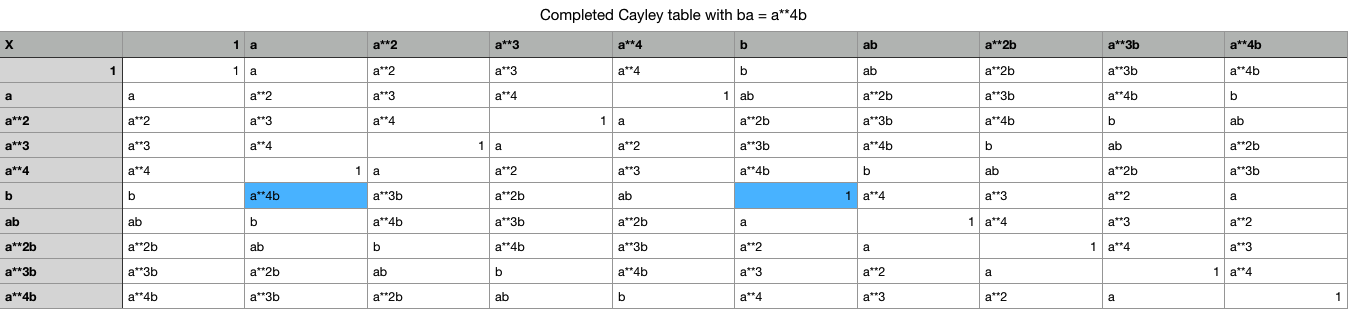
\includegraphics[width=\textwidth,height=2.5\textheight,keepaspectratio]{cayley.png}
  Using this cayley table we can show that there is only the cyclic abelian group $ {Z_{10}, +} $ and the non-abelian group presented in the cayley table.  Thus, only 2 groups of order 10 exist.
\end{enumerate}



\end{document}
